\section{Evaluating Models} \label{evalmodels}
\todo{shorted this}
A number of different machine learning algorithms were used, and the \textit{accuracy} for each model was calculated as an estimate for it's overall performance. Accuracy is defined to be the proportion of correctly predicted instances to the total number of predictions:
$$
accuracy = \frac{tp+tn}{tp+tn+fp+fn}
$$
where $tp$ and $tn$ are true positives and true negatives, and $fp$ and $fn$ are false positives and false negatives respectively \cite{vanwinckelen2012estimating}.
%These parameters are the different types of outcomes that can occur in a classification problem, and can be visualised in a confusion matrix, as shown in Figure \ref{cmatrix}.

\begin{comment}
\begin{figure}[ht]
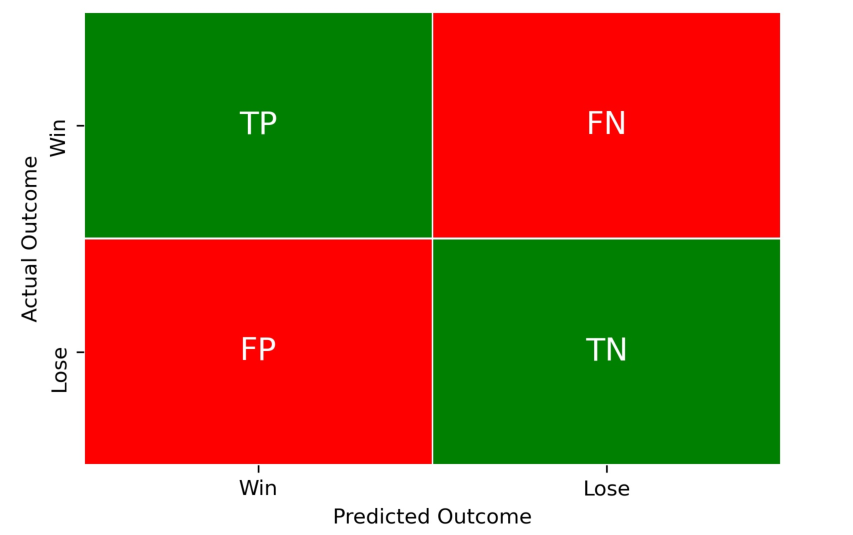
\includegraphics[width=8.5cm]{plots/confusionmatrix.pdf}
\caption{Confusion matrix comparing actual to predicted values}
\label{cmatrix}
\centering
\end{figure}
\end{comment}

\sophie{should figures 2 and 3 be kept?}
\denes{No, but we could report all the confusion matrices for each model (possibly in the appendices).}
Additionally, \textit{precision} and \textit{recall} were calculated for each model. Precision is defined as the proportion of true positives to the total number of predictions predicted positive, and is a percentage of returned results which are relevant. Recall is defined to be the proportion of true positives to the total number of actual positives, and is a percentage of relevant data which have been correctly classified \cite{buckland1994relationship}.
$$
precision = \frac{tp}{tp+fp} \\
\quad recall = \frac{tp}{tp+fn}
$$
Both metrics are important to take into consideration, and ultimately a model's \textit{F1 score} is calculated, which can be interpreted as the harmonic mean between precision and recall. This value is best at 1, and worst at 0.
$$
F1 \ score = 2 \cdot \frac{precision \cdot recall}{precision + recall}
$$

An issue associated with training models is the possibility for the model to \textit{overfit}. Overfitting occurs when a model captures unwanted bias and noise in the data that it negatively impacts the performance of a model. The model corresponds to it's initial training data too well, and fails to predict unseen data reliably. In order to limit overfitting, a popular re-sampling technique called $k$-fold cross validation is used.

In cross validation, the dataset is split into $k$ random subsets, known as folds, and one is selected as a test set for the model to test on, while the others are used as a training set for the model to train on. This is repeated $k$ times where a different subset of data is used as the test set each time, and the overall performance of the model is calculated as the average of accuracy scores for each iteration \cite{berrar2019cross}.
%(see Figure \ref{crossval}).

\begin{comment}
\begin{figure}[H]
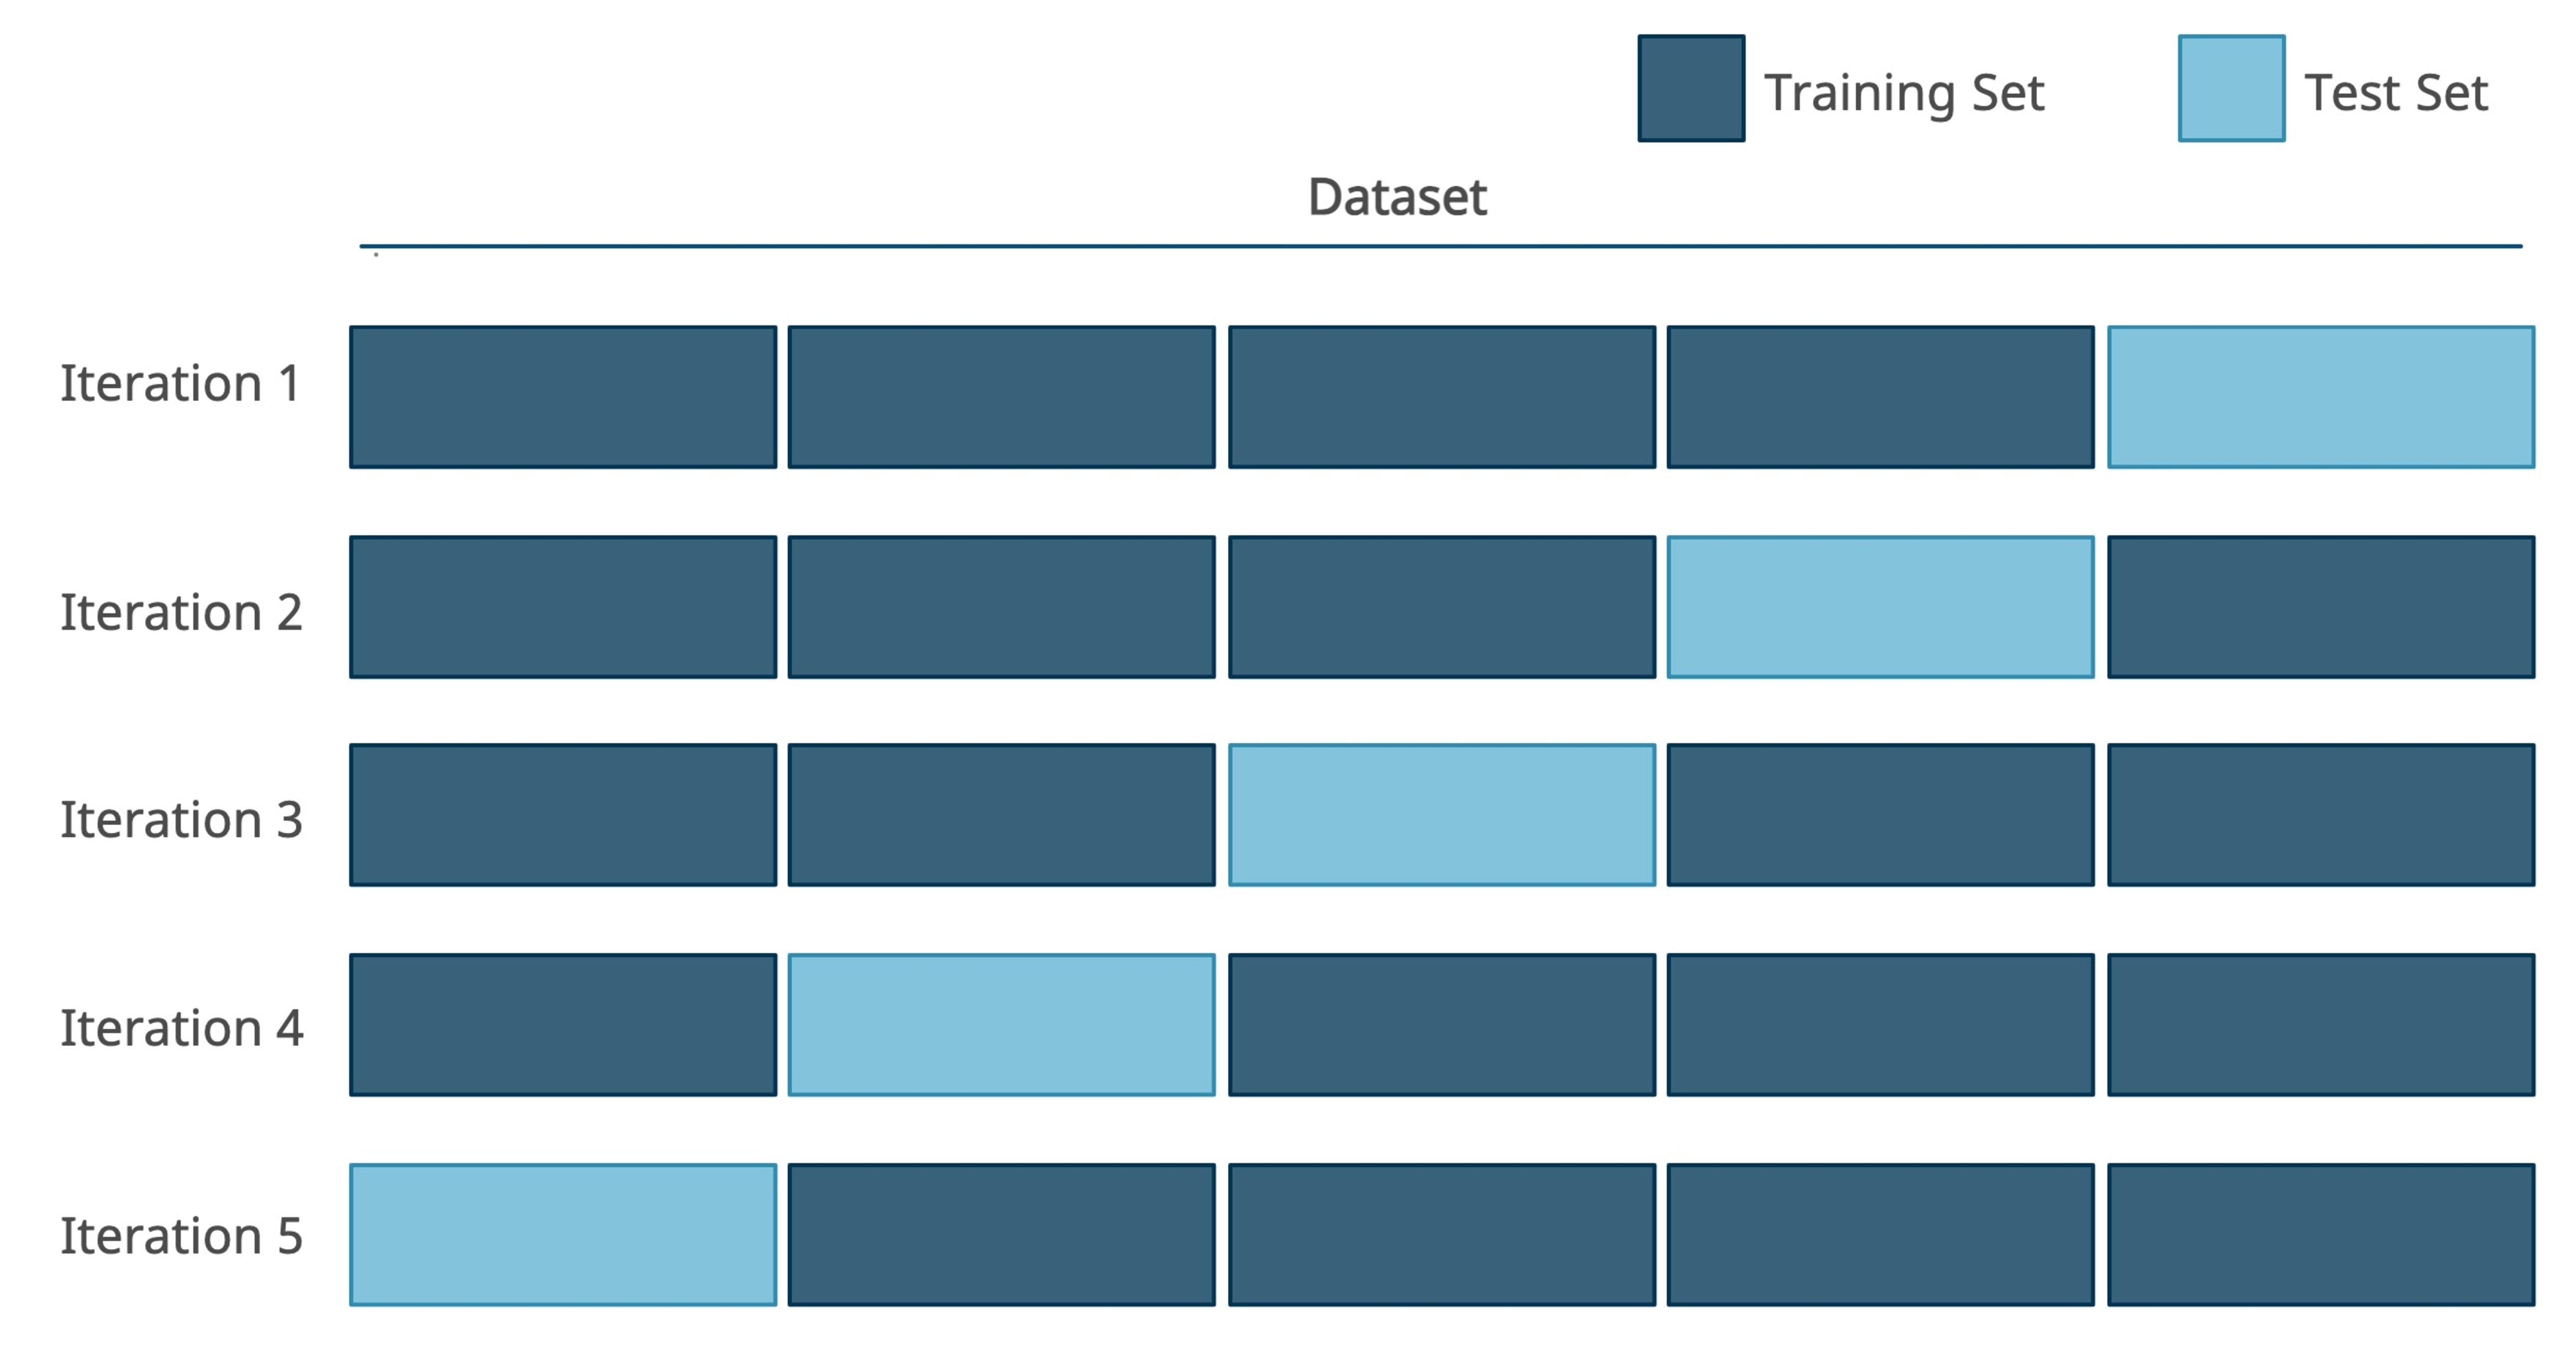
\includegraphics[width=8.5cm]{plots/crossval.pdf}
\caption{How data is split for $k$-fold cross validation where $k=5$}
\label{crossval}
\centering
\end{figure}
\end{comment}

\section{Experimental Results} \label{experresults}
The whole dataset was split in a ratio such that there was a training set, validation set and test set. 10\% of the original dataset was used as a test set, and of the remaining 90\%, the data was split in an 80:20 ratio for the training and validation set.
The model trains on the training set, and the validation set is used for optimising the hyperparameters of the model. The best combination of hyperparameters for a model is determined by whichever has the highest accuracy on the validation set using 5-fold cross validation.
The test set is completely left out from the training process of the model, and is only used during evaluation. This is to see how well models generalise to unseen data which replicate new match data, as the test set is never used before evaluation. During evaluation, all other data is used for training the model (training and validation).
Both accuracy and F1 score is reported for the validation and test sets. The standard deviation for each score for the validation set is reported as a basis of defining uncertainty; the results are shown in Table \ref{results}.

\begin{table}[H]
\caption{Model performance comparing validation and test sets}
\label{results}
\centering
\setlength{\tabcolsep}{3pt}
\scalebox{1.05}{%
\begin{tabular}{ l|c c|c c }

\multirow{2}{4em}{Model} &
\multicolumn{2}{|c|}{Validation set} &
\multicolumn{2}{|c}{Test set} \\
\cline{2-5}
  & Acc & F1 & Acc & F1 \\

\hline \hline 
Logistic Regression & 0.699$\pm{0.053}$ & 0.705$\pm{0.052}$ & 0.722 & 0.706 \\
Random Forest & 0.677$\pm{0.071}$ & 0.688$\pm{0.073}$ & 0.667 & 0.684 \\
Support Vector Machine & & \\
$\rightarrow$ Linear & 0.696$\pm{0.064}$ & 0.690$\pm{0.078}$ & 0.639 & 0.629 \\
$\rightarrow$ RBF    & 0.700$\pm{0.056}$ & 0.677$\pm{0.077}$ & 0.667 & 0.600 \\
$\rightarrow$ Polynomial & 0.705$\pm{0.046}$ & 0.685$\pm{0.046}$ & 0.611 & 0.563\\
$\rightarrow$ Sigmoid & 0.705$\pm{0.039}$ & 0.690$\pm{0.041}$ & 0.694 & 0.621 \\
MLP Neural Network & 0.696$\pm{0.043}$ & 0.708$\pm{0.045}$ & 0.694 & 0.703\\
[1ex]
\hline
\end{tabular}}
\end{table}